% This example An LaTeX document showing how to use the l3proj class to
% write your report. Use pdflatex and bibtex to process the file, creating 
% a PDF file as output (there is no need to use dvips when using pdflatex).

% Modified 

\documentclass{l3proj}
\usepackage{graphicx}
\begin{document}
\title{Grammar ToolKit: A Tool for Creating and Editing Grammars}
\author{Phillipa Russell \\
        Nishad Mathur \\
        Rosie Wilson \\
        Bryan Docherty \\
        Henrikas Elsbergas}
        
\date{ March 2015}
\maketitle
\begin{abstract}

The abstract goes here

\end{abstract}
\educationalconsent
\tableofcontents
%==============================================================================
\chapter{Introduction}
This chapter will give provide information regarding the motivation of the project, a description of our project aims, and a brief overview of the reports remaining chapters. This chapter will provide a base for the remaining chapters, allowing later information to be clearly understood.

\label{intro}

\section{Motivation}
Team L is comprised of five students currently studying Computer Science at the University of Glasgow. Our team will be working from September 2014 until March 2015 on this project which is the solitary measure of assessment for the Team Project 3 course. By the end of the 7 month period, the team hopes to provide a fully functioning tool that will fulfil the requirements set out by the teams client. 

Our project is to provide an 'Interactive Grammar Toolkit' in an implementation method of our choice. Our client is Dr Simon Gay, a senior lecturer at the Computer Science department at the University of Glasgow whom taught our team the background information regarding Grammars and their purpose. In addition to our client there are several other possible clients who will be interested in this project: future third year students of the Computer Science department will be able to use our toolkit to further develop their understanding of Grammars; other individuals outside the university interested in developing grammars and future lecturers at our University and others who wish to further their students understanding of Grammars with interactive measures.  The basis behind the toolkit is to implement an easier way for grammars to be developed which does not heavily rely on knowledge of grammar development "black arts".

\section{Project Aims}
The aim of our project was to develop an 'Interactive Grammar Toolkit' for future students of the University of Glasgow and possible external users who wish for an easier way to develop and learn about Grammar development. As a project this has been heavily client dependent and knowledge based, our team has had weekly meetings with our client Dr Simon Gay in order to gain advice and ensure that our high quality solution meets his original requirements. 

Throughout the process we identified the following additional aims to our project:
\begin {itemize}
	\item To develop the tool as a IntelliJ Plugin
	\item To develop the editor for EBNF formatting
	\item To provide users with some feedback coetaneously as development of the Grammar
	\item To provide a variety of visualisers for the grammar
	\item Make the development of a grammar easier than current methods
\end{itemize}
 
\section{Overview}
The dissertation discusses the overall team development behind the Interactive Grammar ToolKit project:\\

Chapter 2 discusses the background behind the project and similar systems that currently exist.\\
Chapter 3 discusses the design in terms of project requirements,decisions made and project timetable.\\ 
Chapter 4 discusses the implementation of the project and team organisation.\\
Chapter 5 discusses the testing process used and evaluates the final product in comparison with original design plans.\\
Chapter 6 concludes the dissertation and discusses potential future work that could be done to the project.\\
\\
Following from this will be the appendices which include the following:
\begin {enumerate}
	\item \textbf{Source Code} : the source code of all files and classes implemented in the project
	\item \textbf{Instruction Manual}: the Instruction Manual, covering how to install the product, using the product and troubleshooting.
\end{enumerate}

\section{Preliminaries}
In order to fully understand and enjoy this report to the greatest possible extent, some background knowledge is required. The interesting summaries that follow will provide any reader with some background in computing science to comprehend the significance of this report.\\
\\
Regardless of your previous knowledge regarding grammars and their purpose, it is worth researching the role a grammar plays in a programming language. A Grammar is the set of rules which lay the framework of the entire programming language whilst providing structure and laws regarding the programming languages use. It is very similar to a spoken languages grammar and defines how the programming language appears to the user and how it is translated into a machine readable format. Defining your grammar correctly is one of the most important stages in developing a programming language as it plays a key crucial role ; meaning that it can be difficult to change if a mistake is uncovered and can lead to a incorrect Abstract Syntax Tree (AST) for your language. \\
\\
Lexers and parsers both make up syntactic analysis whose purpose is to check that the source is well-formed and determines it's overall structure. The lexer breaks the source down into individual tokens which are then passed to the parser which determines the structure of the source based on these tokens. A lexer itself can be divided into two stages: the scanner, which segments the input sequence into groups and categorizes these into token classes; and the evaluator, which converts the raw input characters into a processed value.
\\
IntelliJ is a development environment that is very popular amongst program developers. It allows users to develop their own plugins to enhance and personalise their use of the environment. This method allows any user of the software to share the plugins they create, to the extent that there is instructions explaining the steps for developing them. IntelliJ's adaptability makes it very popular, as it can program in a variety of languages meaning that users do not need to change their work IDE to write a program in an alternate language.\\
\\
IDE, Integrated Development Environment or Interactive Development Environment. This is a software application that allows software developers to program, normally in either a specified language or multiple. These applications normally allow multiple programming language support through plugin installation. This allows users of such systems to personalise their work space, however not all IDE's allow for programming in all languages. As such further plugin development is required for some IDE's but they may not fully support the options. IDE's can often include additional options such as version control systems and additional tools like a graphical application appearance for GUI development assistance.\\
\\
JFlex is a scanner generator, also known as a lexical analyser generator, which was written in Java for Java programs. It is a Java rewrite of JLex , and is used to develop and write Lexers for programming language development. Learning this language is a requirement for developing the toolkit. \\
\\

%\begin{figure}
\begin{center}
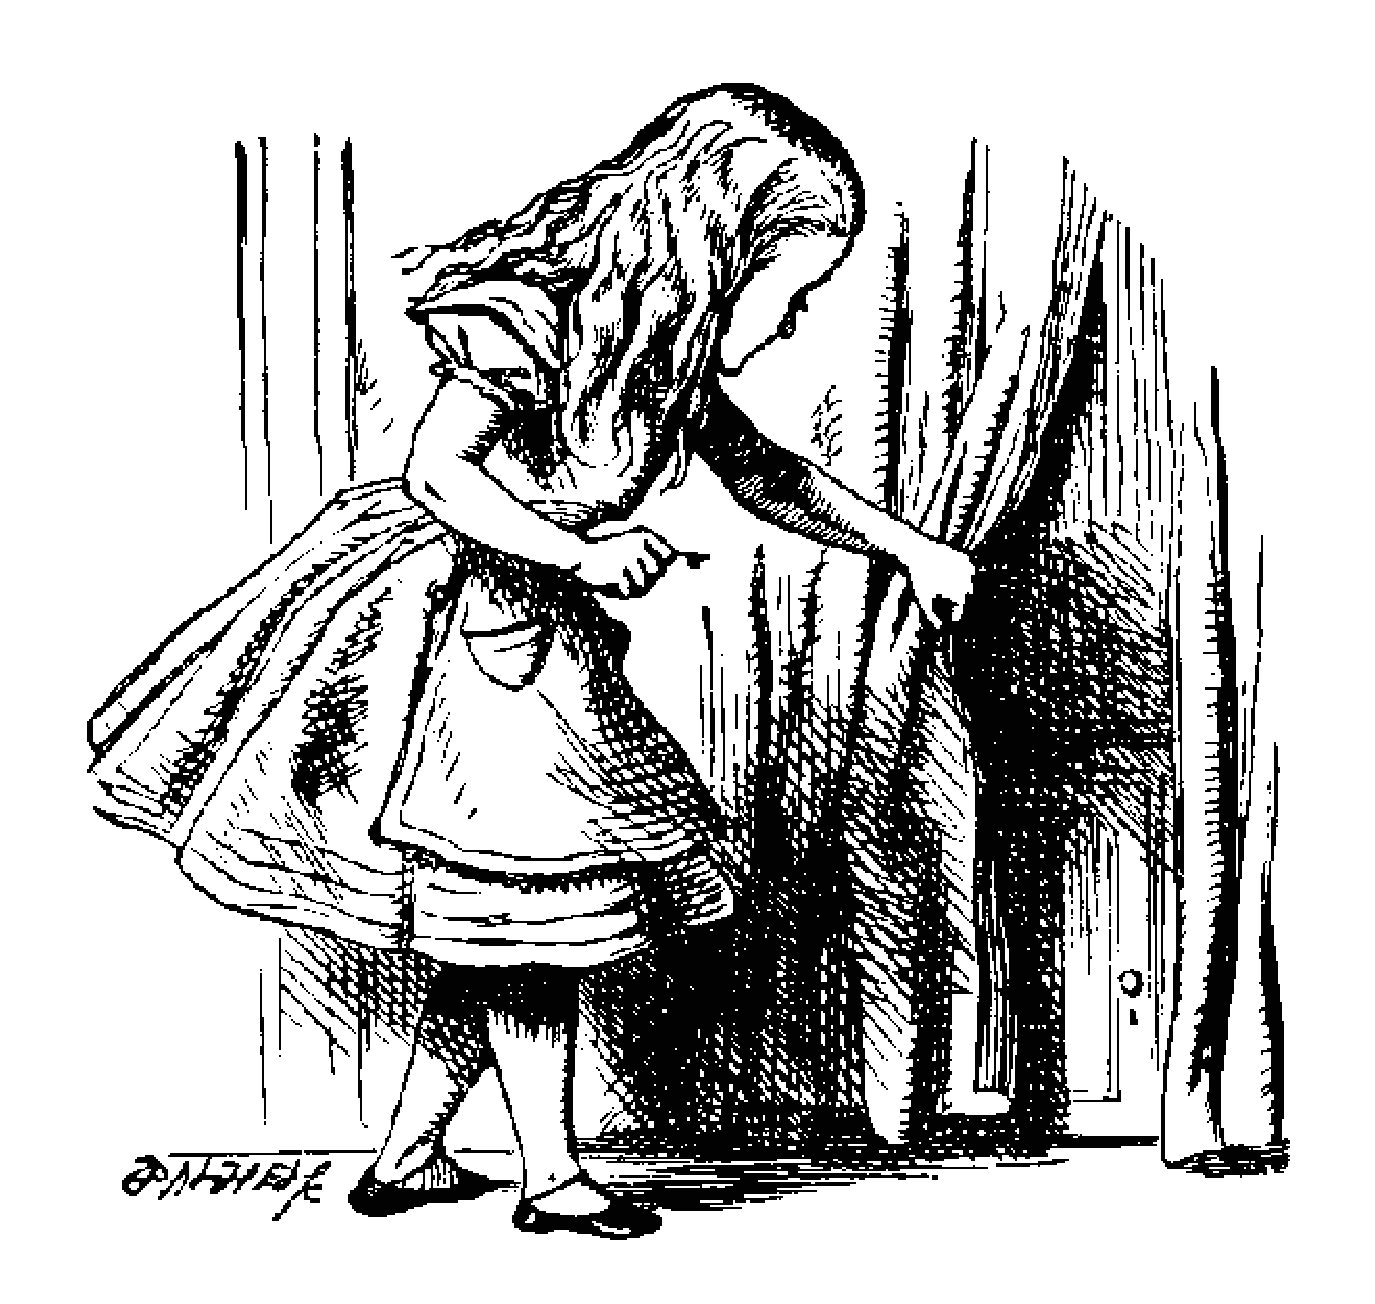
\includegraphics[width=7cm]{figures/alice}
\end{center}
\caption{Behind it was a little door}
\label{fig:alice}
\end{figure}

%\chapter{Background} %haven't done much in this cause i'm not sure how much room implementation and testing will take

%==============================================================================
\chapter{Design}
\label{design}
This chapter discusses the initial client interview, projects requirements and design decisions. Our main decision was to implement our project as an IntelliJ plugin, meaning we didn't need to implement the graphical interface or make significant design decisions beyond the plugins purpose.  However this meant that we were limited in terms of our design options and restricted our first steps to setting up the plugin.\\
\\
\section{Client Interview}
The project was proposed by Dr Simon Gay, a senior lecturer at the University of Glasgow School of Computing Science. Initially, we met with Dr Gay in order to gain more specific information regarding the requirements and specification for the interactive toolkit to ensure that we produced a project within our clients guidelines.\\
\\
Our initial requirements for the toolkit are as follows:
\begin{itemize}
	\item An interactive toolkit that allows users to edit and create Grammars.
	\item Some simple example sentences to show the user how the programming language will work.
	\item Could include a library of normally included grammar sentences.
	\item Our team has the freedom to include whatever features we think will be useful in the toolkit
\end{itemize}

In the initial meeting with our client we discussed possible features to implement in the toolkit. Our team members each investigated some choice features such that they could be discussed with our client the following week in greater detail. One of our main additions we thought would be useful if the toolkit warned the users of left recursion in their grammar. We discussed this idea following the initial client meeting and our client agreed that such a feature would be extremely useful. The functional requirements were then updated to include left recursion support.\\
\\
Following from the initial meeting with our client, we arranged for weekly client meetings in order to update him on the process we had made from the previous meeting. This allowed us to receive guidance on new ideas or features we had considered as well as receive feedback as to our progress. 

\section{User Case Diagram}
Not long after our initial meeting with our client, our team sat down and discussed what our User would need to be able to achieve when using our plugin. We discussed the necessary things our plugin would need to allow, and the optional features we may with to implement. This lead to our Project Specification creation,by combining our initial designs with our client interview information, and the researched documents we found online. Our discussions covered what we wanted Users to be able to accomplish when using our base plugin, which then lead to the features we personally would like to add for additional usability from the users point of view. The initial diagram was redrawn using digital software, and can be found below [Figure 2.1]:

\begin{figure}[ht!]
\centering
\hspace*{-2.5cm}\includegraphics[width=\paperwidth]{figures/user_case_diagram.jpg}
\caption{User Case Diagram for our project \label{overflow}}
\end{figure}

As seen in Figure 2.1, we decided the main tasks the user wished to complete were as follows:
\begin {itemize}
	\item Create a New Grammar: The user must be able to create a brand new grammar with our toolkit. This was derived straight from the project specification and is a key goal to completing the plugin.
	\item Load Grammar: Our user must be able to load a previously saved grammar so that they can alter and edit it.
	\item Save Grammar: Our user must be able to save their grammar to their local disk such that they can later use the 'load' function to edit, and such that they can share their grammar code with others.
	\item Edit Grammar: Our user must be able to load the grammar in read-write mode such that they can not only see what they have previously done, but alter current code as well as add new code to the saved grammar. 
	\item Export Grammar: Our user must be able to export the grammar in a format that means it can be parsed by commonly used standard parsers.
	\item See Diagrams: Our user must be able to see diagram representations of their grammar, to help them understand the actions their grammar is taking. 
\end{itemize}
All of the above actions are necessary tasks we wish our user to be able to complete upon using our program. This section of the User Case Diagram (Figure 2.1) was discussed with all team members to ensure that everyone was aware of the base jobs the toolkit was required to achieve from the users point of view.  From this we then started discussing extraneous features that we may wish the user to be able to achieve upon using our project. 

\begin {itemize}
	\item Left Recursion Support: This was brought up in our original client meeting as a possible addition to our project. It would allow our toolkit to inform the user when the are using left recursion in their grammar, and possibly remove or correct it for them. At this stage we have no knowledge of the level of difficulty that implementing this feature, as such it is an optional feature with the potential to be required later.
	\item Sample Grammars: it was mentioned in the original interview that we could possibly implement sample grammar code that the user could insert into their own. Implementing this will be restricted by our chosen distribution method (See Decisions), as such it may not be possible to add this feature.
	\item Preview code: our client suggested that we could possibly add the option for the user to see possible code samples that are generated from their grammar. Again this will be restricted by the difficulty and the distribution method, hence why it is currently listed as an optional feature that the user may wish to use.
	\item Reformat code: this is a suggestion one of our team mates suggested. Current popular IDEs allow users to reformat their code to suit their own coding style. As such if we are to develop our toolkit as an IDE, it would be wise to add reformatting tools for our users.
\end {itemize}

The above tasks are all suggested ideas that we could possibly implement depending on our design decisions and level of difficulty. The User Case Diagram was designed to guide our later development of our project, such that we did not forget the main goals of our toolkit once we reached the point of adding additional features. The diagram then allowed us to develop the project specification by deciding how to complete our tasks from a technical point of view.

\section{Project Specification}
This section covers the Project Specification (or spec), which is a comprehensive description of objectives for our development project. It contains all goals, functionality, and details we believe are required to fulfil the requirements of our client. It also covers the decisions we made in order to complete the design of the project. \\
\\
\subsection{Feature Specification}
This section covers the required objectives to complete the project and the optional features we had decided on. \\
\\
\subsubsection{Required Specification}
The aim of our project is to develop a tool and/or plugin which will allow users to edit and create grammars. Grammars created by the tool will use EBNF notation and will be exported from the tool into a variety of languages which can be imported into a selection of external language parsers. The tool will also display examples of programming syntax from the created/edited Grammar. After careful consideration and thorough research, it was decided that the  tool would be implemented as an IntelliJ plugin (see Decisions). The required features for the plugin tool are explained below. 

\begin{enumerate}
	\item \textbf{Registering a file type}: This is the first step in creating the plugin. It tells IntelliJ what file types can be loaded with our plugin and allows us to set-up our own individualised file type that can only be used by our plugin for the user to work on before exporting it, for example C programs being written in .c files before being compiled into .out files.
	\item \textbf{Implement a Lexer}: this will define how the grammar file contents are broken down, for example "2 + 3" is recognised as 2 numbers with 2 white-spaces and a plus symbol. These symbol definitions will then be fed into the parser to create a syntax tree(see Parser). This is not only necessary for the plugin, but will allow us to provide a lot of extra implementation later on.
	\item \textbf{Parser}: a parser must be provided to talk to the lexer and develop an abstract syntax tree(AST). The AST tree will give combinations of allowed syntax based on the lexer information, for example with the lexer data (see Lexer) the tree would state that a file can have a math expression that can have a number, a plus symbol, followed by a number (some languages are not bothered by spaces). This parser is for our plugin and BNF, it will not parser the grammar files the user creates. The created AST tree covers the range of text that can exist in the document.
	\item \textbf{PSI(Program Structure Interface)}: this will work with the parser to create a second tree (a PSI tree) on top of the AST tree which will compliment it by adding ways for the user to alter the language, for example with our math expression you can change the numbers all you wish. 
	\item \textbf{Syntax and Error Highlighting}: this will allow the user to highlight pieces of text as one would in a text editor to make it easier to copy or delete pieces of text. It will also highlight errors in the grammar as the users type similar to a text editor underlining mis-spelt words.
	\item \textbf{Fixits and Compatibility warnings}: The system could be capable of detecting problematic constructs eg. left recursion and offering potential solutions to the problems, eg by refactoring the system into a right recursive function etc. This could also be implemented to detect unmatchable rules and potentially highlight overly broad rules that are not very specific in terms of common grammar notation. However both of these features would require more research and are dependant on the remaining time available. 
	\item \textbf{References}: this is a requirement of the plugin. One of the main features of IntelliJ is that the user can use a keyboard shortcut to go from the usage of an element (such as a variable or function) to their declaration. This will make the plugin more user friendly.
	\item \textbf{Find Usages}: this feature is the opposite of the previous one. It will allow the user to search the file for all usages of an element, before getting to view all options at the side similar to pdf searching.
	\item \textbf{Refactoring}: If time permits after implementing our planned main features,then we will try add any other refactoring features that we can think of, but this needs some extra research before we finalise it due to the specalised nature of these features. Some possible options include:
	      \begin{itemize}
		    \item Rename : This will allow users to select the declaration of an object and rename it across the entire grammar, for example renaming A as B will replace all A in the grammar with B. This will make our tool more user friendly as it will allow users to change their grammar more easily. 
		    \item Rule Generation: This is a variation of autocorrect, where the plugin will attempt to predict what the user is trying to type and suggest an alternate 'correct' version, for example in text documents when typing an incorrectly spelt work, a tooltip will appear with the correct spelling.
		    \item Extract subrule into a separate rule: this feature will allow the user to easily make a subrule into a seperate rule without needing to complicate or potentially break their grammar. 
		    \item extract regular expression/string into token etc.: this covers a variety of features which may or may not be suitable for our planned implementation. Refactoring covers a variety of tools and tasks which users do not realise are all covered by refactoring tools.
	      \end{itemize}
	\item \textbf{Diagrams}: Railroad diagrams and if time allows syntax diagrams of example expressions. We are planning on having railroad diagrams generated from the EBNF and then, giving the option to view the diagram inline in the program, or exporting it as a png (or similar). 
	\item \textbf{Source Converters}: These will take out BNF file and then convert the file into an AST then output them into the output formats, currently we're looking at:
	      \begin{itemize}
		    \item ANTLr
		    \item JFlex/CUP
		    \item GrammarKit
		    \item Yacc
	      \end{itemize}
	      
	\item \textbf{Left Recursion}:  This was originally an optional feature. Upon discussion with our client we decided to add it to the Required items as it is an incredibly difficulty area of grammar creation for learners. The purpose of this feature is to add support for left recursion to the grammar toolkit. This will inform users if their created grammar has left recursion present. 
\end {enumerate}
We felt we required further research to decide exactly where we go from here. Tighter integration with the parsers would be nice, but needs more work, eg could automatically download and setup the jars etc for each tool to simplify setup.

\subsubsection{Optional Features}
\begin {enumerate}
	\item \textbf{Source templates and generators}: for example
	  \begin {itemize}
		\item Operator definition and precedence definition : This could either be a static template, or a macro like construct, or perhaps something similar to Swifts operator overloading system.
		\item Simple grammars in various formats eg: Maths grammar, basic python like grammar, basic java
		\item Common syntax constructs such as: linebreaks, identifiers, comments (eol and block), strings, basic operators
		\item Could be done as an importable library, or as generated code. An import system could be handy in other ways eg only import part of a grammar.
	  \end {itemize}
      \item \textbf{Sample + Grammar = Graphic visualisation}
	  \begin {itemize}
		\item A way to view how the system actually parses an expression into an AST, how each section is classified etc. Potentially something similar to the what was shown in class.
		\item It could support similar export functionality to the railroad diagrams.
	  \end {itemize}
      \item \textbf{ A Preview Editor }
	  \begin {itemize}
		\item Ideally this would be a way to enter full examples (not just snippets) of a program and view the full AST and error highlighting etc of the program, with the ability to see the tokenized version of the sample and why certain samples are not being parsed correctly etc.
		\item Something similar to the GrammarKit plugin or similar to Xcode Playgrounds would be nice here (or some form of repl).
	  \end {itemize}
      \item \textbf{Source Maps} : So we can map errors in the generated code back into our own syntax, and then highlight them for the user. Would enable tighter coupling with the and parser generator. (This would also highlight ambiguous grammars etc).
            \item \textbf{Basic testing framework}: Define a list (or w/e) of samples/snippets and verify that they are (or are not)  valid samples of the grammar. Potentially this could verify individual rules instead of the grammar in general, but that needs further investigation.
            \item \textbf{Source Reformatting}: Have the IDE reformat the code into a standard/predefined format automagically, either on save or on request.  Could be integrated into the exporters, or use the intellij source code formatting framework.

\end{enumerate}




\section{Decisions}

In order to successfully develop the tool, we were required to make some decisions regarding how to go forward with implementation. Such decisions are covered in detail in the following sections. All decisions were thoroughly research and discussed with team members before a final decision was made. In the following sections, each options pros and cons are offered before an explanation of the decision and the reason behind it are given.\\
\\ 

\subsection{Deciding on roles}
In the first few weeks of the project we needed to decide what roles each team member would take on.  This was based on each team members previous work in all projects. In order to decide each team members role for the project, a variety of steps were under taken:
\begin {enumerate}
	\item We needed to establish each team members individual's skills and decide how to apply those skills to the team project.
	\item We discussed each team members previous projects in order to establish previous roles so that those team members could apply previous role knowledge in the current project. 
	\item After careful consideration of all team mates skills and previous project knowledge we established which roles would be perfect for our team. This allowed us to firmly lay the groundwork for our project as each member had specific roles they would need to complete.
	\begin{enumerate}
		\item Phillipa Russell: Secretary : This team member had previous taken a course in dissertation writing and documentation. As such her main job in the first semester was to keep track of all duties that were performed during the project and of all team meetings. In the second semester her job was to correlate all previous documents with new information in order to write the dissertation.
		\item Nishad Mathur : This team member was the main previous user of IntelliJ, as such their main job was to research the needed plugin features. Due to previous project experience, this team member was also selected to be in charge of the programming  sub-team whose members varied as time progressed. 
		\item Rosie Wilson : This team member had a lot of previous experience with testing applications, as such they were selected to be in charge of the eventual testing of our plugin. During the projects iteration, this team member was also to assist in documentation and be an occasional part of the programming team when other tasks were completed. 
		\item Bryan Docherty : This team member was chosen to be the customer liaison. It was his job to contact our client, Dr Simon Gay, whenever a problem arose or to re-arrange a meeting. This team member was also assigned to be part of the programming team.
		\item Henrikas Elsbergas:This team member had the most experience of large scale projects as such he was assigned to create the overall design for the plugin,  as well as being a constant member of the  programming team  as both a programmer and a quality assurance personnel.
	\end{enumerate}
\end{enumerate}

These team roles were gladly accepted by all team members due to the thorough research conducted. The discussion into all team members previous skills and project experience meant that the development of the project would develop more smoothly since all team members were aware of every other members abilities and limitations.\\
\\

\subsection{IntelliJ Plugin or Develop own IDE}

One of our major decisions in the initial weeks was considering the type of tool we would develop. After discussion and research, we narrowed our decision to two options: develop our own IDE, or develop an IntelliJ plugin.  All feasible options would require new knowledge and skills not currently known by any members of the team. These factors, and all of the following discussed below were taken into consideration to make the final decision.
\\
\subsubsection{IntelliJ}
This briefly overviews the advantages and disadvantages of implementing the toolkit as an IntelliJ plugin, with a brief summary overview at the end.\\
\\
\textbf {\underline{Advantages}}\\
Given the popularity of the IntelliJ program, there are ample instructions online explaining how to develop a basic plugin for the development software. As such developing the basic plugin base will be no problem even though none of our team member have developed a plugin for this software. As such developing the plugin will be a matter of following the instructions. In addition to this is the amount of online assistance available due to the popularity of developing plugins for IntelliJ. The majority of developers, when they run into a problem, will search online to find if other individuals have found the same problem. Therefore, due to the popularity, any problems we discover will probably been discovered by another developer who will have posted their solution. \\
 \\

 There are currently existing plugins for IntelliJ that perform a slightly similar task.  These plugins are far more specialised than the plugin we are trying to develop, however they prove that IntelliJ can be used for such a project. It also allows us some benchmark programs that we can base our own design on. By using these other plugins we can discover if our way of developing the required features will be viable. It may also allow us to discover features that we had not considered and different methods of developing the features. The specialised nature of the other plugins will not provide us much assistance with the majority of our planned plugin features, but it is worth looking into the other plugins in case they are helpful as it may save us time later in the development.\\
 \\
 In order to develop the plugin, we need to create a variety of features that we will need to develop regardless of our chosen project implementation method. If we chose to implement the toolkit as an IDE (see below) we will still need to implement all the steps required to create the plugin. Implementing them in this method will give us more support and guidance, as well as making the overall process easier and thereby quicker due to the IntelliJ plugin development support. The plugin will require set features which will automatically give our plugin additional features we had not considered. \\
 \\
 \textbf {\underline{Dis-Advantages}}\\
In order to develop the plugin for IntelliJ all members of our team would need to learn a new language. As such this could cost much needed time and could also cause complications due to lack of natural knowledge or teaching in the language. The language we would need to learn is called JFlex, which would be needed to develop the lexer for our grammar.\\
\\
We would also need to learn new techniques and further our knowledge of IntelliJ plugins which will only be needed for this project unless we specifically decide to work on IntelliJ plugins as well.\\
\\ 
In addition to this is the fact we would not be allowed to develop any alternate design to suit our project, we will be stuck to the limitations of the IntelliJ framework. As such it would stifle our creativity by refusing to allow us to develop our own graphical user interface. \\
\\
We will also be forced to add features not needed in the IDE option in order to develop it as an IntelliJ plugin. As such we will be required to implement extra features that would cost time in comparison with the IDE option. \\
\\
 \textbf {\underline{Summary}}\\
 Overall the IntelliJ plugin option would save us some time overall due to the previously mentioned instructions and benchmark plugins. Even with the extra features required to implement the plugin, the IntelliJ plugin would save time as no graphical user interface would need to be designed or developed. As such, the saved time from developing the interface can be spent on the extra features only required by the plugin.
 
\subsubsection{IDE}
This briefly overviews the advantages and disadvantages of implementing the toolkit as a self-developed IDE, with a brief summary overview at the end.\\
\\
 \textbf {\underline{Advantages}}\\
Developing the IDE would allow us to freely choose the programming language to develop the program in. As such we could choose the language that the majority of our teammates know and feel confident about, allowing us to swiftly deal with any problems that occur due to our previous knowledge of the language. There is also the fact we would have no need to learn excess languages since we would have the freedom to choose our own programming language. \\
\\ 
All of our teammates have previously done graphical user interface work like this in our previous university projects. All teammates have experience of developing such an program allowing us to equally distribute the workload far more easily since all teammates have experience of all areas of such a project. It would also allow us the freedom to design our own graphical user interface, whereas the IntelliJ plugin would use the IntelliJ interface automatically.\\
\\
 \textbf {\underline{Dis-Advantages}}\\
Developing our own IDE will require more work in comparison with an IntelliJ plugin.Developing such a thing will require us to design the graphical interface from scratch which can be troublesome regardless of programming language chosen to implement the project. In addition to this we would need to fully design the entire project design from scratch which would require extra time. In comparison the IntelliJ plugin has instructions for designing a base plugin for IntelliJ meaning we would only need to design the specific features for our project. Designing our own IDE would mean designing the full user support and back end.\\
\\
There is also no support available beyond our interviews with the client, meaning that there is no help if we run into a problem. As such the entirety of our project will be from scratch which will cost valuable time if we initially make an error in our design in the initial weeks of our project it would be incredibly difficult to correct. This is especially a concern given that none of our teammates have worked with grammars in the past, so developing a toolkit to allow creation of grammars will undoubtably result in errors.\\
\\
\textbf {\underline{Summary}}\\
 Overall the IDE plugin option would allow us total freedom in developing the toolkit, allowing us to choose everything from programming language to the colour of the buttons on screen. However with no documentation available and due to the amount of features we want to ad, the time spent designing the IDE would limit what we could add later on. As such, the cost of total development freedom may very well cause us to run over-time or loose a lot of planned features.

\subsubsection{Overall Decision}
In light of the advantages and disadvantages, our team decided to implement our toolkit as an IntelliJ plugin. While this means sacrificing design privileges and causing our project plan to be limited to the development of the base plugin, it will allow us to add more features to our toolkit, thereby making it more useful to a wider variety of users.\\
\\ 

\subsection{Including left recursion}
Our team had to decide if we would include left recursion support within our Grammar developer. Had to decide whether to include support for left recursion or not. This was due to some parsers supporting left recursion and some not. Rosie and Bryan were tasked with researching how easy this would be to implement and the various ways we could implement it. This weighed heavily on our decision as to whether to include it or not, as these methods difficulty would affect the implementation time which would put everything else back. We decided to implement it, based on Rosie and Bryans findings which supplied a variety of methods to suit our parser.




\subsection{Using strings in parser}
(-talk to nishad about) %might leave this out as decision section is big enough already, what do you all think?


\subsection{Communication method}
In the early days of the project, we needed to decide what communication methods and meeting times would suit everyone. This was an important decision as it would affect how much information we could exchange outside the lab and affect how likely we were as individuals to use the chosen method.\\
\subsubsection{Facebook}
\textbf {\underline{Advantages}}\\
\\
Facebook has recently increased in great popularity in past years, as such there is a great chance our team members already have accounts for it. This will limit problems for our team members in trying to set up accounts for communication methods we will only use for this project. It will also limit our team members having to give private information to companies and communication sites that we may not wish too.\\
\\
Currently Facebook has the messenger function available as a separate application that can be used in order to keep our work separate from our normal personal uses of Facebook. Facebook also allows to create our own group page for permanent communications such as links to documents and information announcements. As such we can not only reach our team mates using the messenger app, but can also use the group page to inform all team mates of something important, giving us a place to discuss the project and a separate 'noticeboard'. \\
\textbf {\underline{Dis-Advantages}}\\
\\
It is not the preferred method of communication for all of our members, regardless of them having accounts. As such those members may not initially be used to checking Facebook for updates from team members. This may delay our project progress as all team members may not be receiving the same level of information regarding tasks that need completion. As such this problem will need to be addressed such that all team members can receive the same level of information. \\
\\
Facebook's Video chat is currently not very reliable. Our team member have attempted to use it, however it has repeatedly removed or members from the video chat and has claimed members are online when they are in fact not. Also the Facebook video chat feature is not available on the website, it is only accessible through the separate messenger application that cannot be downloaded on computers. As such, if we wished to video chat Facebook would not be a viable option for our team members.\\
\\
\textbf {\underline{Summary}}\\
\\
Facebook is a popular communication method that will allow us to have a private group chat that we can separate from our personal interests, as well as allowing us a group page to post notices on. However, not all team members are fond of Facebook and the current communication method is restricted to text chat as the video chat option is not operational to the level we require.\\
\\
\subsubsection{Skype}
\textbf {\underline{Advantages}}\\
\\
Skype has now been combined with hotmail messenger, as such our team members would be able to use their Microsoft account to communicate in a text format, as well as communicate using skips call feature and video calls. This would prevent our team members from needing multiple accounts, as all possible communication options are available with one account. This is preferable to our team members as it means they will only require knowledge of one account and will allow them to receive all messages related to the project from one source.\\
\\
Skype is very popular for video conferences as it allows free video chat across the internet. This is a very popular feature with our team members as there is the possibility of team members being ill in future weeks, or possibly being abroad. This would allow our team members to communicate easily with our team members without physically being present, as a face to face discussion is more preferable for team meetings than communication over text. \\
\\
\textbf {\underline{Dis-Advantages}}\\
\\
Currently not all of our team members have a Microsoft account that is setup for Skype. This will mean extra time spent to set up a communication method that we will only use for this project. It is also added strain on our team members as it is one more application that they need to install and check on a daily basis. This raises the possibility of team members forgetting to check Skype since they are not used to checking for notifications from there.\\
\\
Since all possible communication methods (text,phone,video chat) are available through Skype, there is the possibility that Skype mentally becomes the application we associate with our project, meaning that we are less likely to want to use it for personal use. This may be a problem for those team members who currently use Skype for personal use. It may also become a problem as if one team member becomes locked out of their account, they will not have any way of communicating to our team members that they cannot access their account since all communication methods are in one application. \\
\\
\textbf {\underline{Summary}}\\
\\
Skype is a popular communication method that allows us to have all forms of communication under 'one roof' so to speak, with a video conference option that has received raving reviews. However, only 2 of our team members currently have a Skype account, with only 1 of them actively using Skype so the transition to use it could cause difficulties. The one account option also raises the possibility of a team member being unable to contact the team due to either being locked out of the account or not being able to reach Skype servers.\\
\\
\subsubsection{Overall Decision}
Overall we decided to choose Facebook as our main communication method, with Skype as our backup method. This allowed us to have the separate sections for personal and work, as well as having the group 'noticeboard' page alongside our communication chat. Having Skype as a backup means that we can take advantage of its superior video chat option whilst giving our team members a way to communicate that they are currently locked out of Facebook. \\
\\

\subsection{BNF vs. EBNF}
At an early stage we were required to decide what type of grammars we would allow users to write, either grammars written in BNF or grammars written in EBNF. BNF stands for Backus-Naur Form and is a standard language for writing grammars in. EBNF stands for Extended Backus-Naur Form and includes all of the BNF notations along with extra options which make is easier for grammar development. We had to research and weigh up the advantages and disadvantages of each option, which are expressed as follows:\\
\\
\subsubsection{BNF}

\textbf {\underline{Advantages}}\\
\\
 Initial investigations indicated that implementing the toolkit for BNF would be simpler and therefore quicker for us to develop. Our research indicated that it would be simpler for us to develop the support for BNF since it does not have as much notation as EBNF. This would free us extra time from development of the grammar language that we could spend on error correction or on developing extra features for our toolkit. The development would also be easier to understand from a developers pint of view due to the limited word range in comparison to EBNF. his would also make other areas of the project easier to implement, for example the erro detection section, as our team would have less to support making the developnent of the backend suport areas of the project quicker to develop. \\
\\
Our client, Dr. Simon Gay, requested a specific feature for our toolkit: a user of the tool must be able to export it from the tool such that a selection of external parsers can parse the user created grammar. As such, if we implemented the project using BNF for the set language, we would have a wider amount of parsers available to implement exportation for. As such we would have the freedom to choose which parsers to implement for, as some would be more complicated than others. This would give us more design freedom and may be quicker in implementation as there may be more support online for developing for those parsers.\\
\\
\textbf {\underline{Dis-Advantages}}\\
\\
One obvious concern is that it would limit the users creativity. BNF has less notation options than EBNF, thereby disallowing users who wish to use EBNF notation from using our tool to develop their own grammar. This is a serious concern as we wish to create the tool such that it can be used by as many possible users as we can manage to implement support for. Whilst EBNF will support BNF, BNF will not support EBNF because EBNF is BNF with additional features, thereby if a user programs the grammar using one of these additional features then BNF will not support it.\\
\\
One of the main differences between BNF and EBNF is that BNF only allows one notation per line. As such users cannot group sections of their grammar together in creation, for example having 'firstname' and 'lastname' notation on the same line for ease of locating and legibility. In BNF this would not be allowed. In terms of implementation this may be slightly complicated once we begin to add features to our tool beyond the basic creation tools, as enforcing the rule may interfere with our suggested features. It will also restrict the user in their own grammar development: the purpose of this tool is to help users learn more about grammars and their creation, without getting 'bogged down' in the confusing rules like having one notation per line. As such by choosing to implement it in BNF we may cause ourselves extra work and problems in later development stages, and we may restrict the users learning ability when using the tool. \\
\\
\textbf {\underline{Summary}}\\
\\
Overall BNF notation will save us time in development since we would need to provide support for less notation rules, and it would allow us greater freedom in choosing which parsers to export too. However it would limit the users ability to create grammars and could potentially damage their learning ability which is one of the main points of the project.

\subsubsection{EBNF}
This discusses the advantages and disadvantages of implementing the grammar tool to support EBNF notation rather than BNF. 
\textbf {\underline{Advantages}}

EBNF as a wider variety of notation available for the user to create their ideal grammar. This will allow our tool to be used by a wider variety of users who wish to create grammars for a greater amount of purposes. The wider notation will also allow our users the ability of writing BNF grammars in our toolkit as EBNF includes all BNF notation, so by implementing EBNF support we will avoid alienating those users who wish to strictly use BNF notation. \\
\\
EBNF supports more user-friendly notation, such as having more than one declaration on a line. This will allow those users who have done other programming before to feel more at home, and will allow those users who are brand new to learn more about grammar creation without getting too involved in programming rules.\\
\\
\textbf {\underline{Dis-Advantages}}\\
\\
EBNF has a greater number and variety of possible notation for users to use in thir grammar when compared to BNF, as such this increases the possibility of developing an error in this crucial stage, since there is more for us to program and potentially program incorrectly. There is also the time concern: the more we are needed to program, then the more we will need to support in other features thereby limiting our potential list of alternate features in the toolkit.\\
\\
EBNF is not supported by all of the parsers. This wil limit which parsers we can export too, which could potentially be troublesome as exporting grammars into a parser friendly format may be varied in difficulty depending on the parser and grammar complexity. As such we may spend more time in the later stages of the project trying to export to complicated parsers because we chose EBNF notation in this early stage.\\
\\
\textbf {\underline{Summary}}\\
\\
Choosing EBNF notation will make our toolkit more useful for users and more user-fiendly by adding extra optional notation and by helping them avoid the strict rules of grammar creation. However, it may cost us a lot of time we could spend on other areas, mainly due to the increased notation and possible complexity of the created grammars.\\
\\subsubsection{Overall Decision}\\
\\
Due to our research and team discussions, we chose to implement EBNF notation. We decided that it was better to provide a tool that could be used by a wider variety of users that was user friendly. We are aware that it may cost us a lot of time due to complexity, and may restrict what features we can add, but our research indicted that any usefulness added by potential features, would not make up the helpfulness lost from not choosing EBNF at this early stage. \\
\\

\section{Project Plan and Timetable}
In the initial few weeks, our team devised a plan for the project for dividing up the work for the next seven months. This was initially devised by creating a list of necessary components that would need to be implemented in order to fulfil the clients specification. Following this , optional extras were added to the list as possible additions to the product that would give extended features to the finalised product

\subsection{Project TimeTable}
The following timetable is our initial project timetable. The timetable was devised by listing all tasks we definitely needed to implement to complete the project. This was then thoroughly discussed and researched by our team members to try and decide how long each of these tasks would take. Due to lack of experience in developing such a plugin we overestimated in some areas in our time calculation, which eventually served us well as it gave us extra time we had not scheduled for to correct errors that occurred. Those items in bold that have a blank entry for 'Days planned' are minor titles within the table, the items following these until the blank line are all covered under these minor titles. 
\begin{center}
    \begin{tabular}{ | l | l |}
    \hline
     \textbf{Activity} & \textbf{Days planned}  \\ \hline
    Define Specs, Initial Organisation & 7     \\ \hline
    Setup Project and Github & 4   \\ \hline
    Learn Git & 7  \\ \hline
    Learn JFlex & 7 \\ \hline
    Register File Type & 2 \\ \hline
    \textbf {Implement Parser,PSI, Mapping References} & \\ \hline
    Implement Parser & 3.5\\ \hline
    Implement PSI & 3.5\\ \hline
    Implement Mapping References & 7\\ \hline
    & \\ \hline
    \textbf{Syntax and Error Highlighting} &\\ \hline
    Syntax & 5 \\ \hline
    Error & 10 \\ \hline
    Annotator & 7 \\ \hline
    Reference Completion & 14 \\ \hline
    Find Usage & 17 \\ \hline
    Refactoring & 8 \\ \hline
    & \\ \hline
    Diagrams & 7 \\ \hline
    User Interface & 4 \\ \hline
    Backend & 3 \\ \hline
    \end{tabular}
\end{center}

\subsection{Optional Features TimeTable}
The following timetable is a secondary timetable we created in order to decide if we could implement additional features. It covers all those features we had discussed with our client and team members as possible extras to improve the functionality of our plugin. The first three items in the optional list are necessary items but they are not needed to complete the physical plugin, hence why they are not in the design functional specification section (Chapter 2 Design). Everything else are optional extras that we may implement if we have time after developing the plugin and if we can implement them without damaging what we have already done. In the following table, those items listed with 'throughout' are those tasks we needed to perform during the length of the project.
\begin{center}
    \begin{tabular}{ | l | l |}
    \hline
    \textbf{Activity} & \textbf{Days planned}  \\ \hline
    Testing & 21 + throughout     \\ \hline
    Documentation & throughout + 7 at end   \\ \hline
    Report & 35  \\ \hline
    Contributor based Completion  & 14\\ \hline
    Find Usages & 4 \\ \hline
    Code Formatter & 10\\ \hline
    Code Inspections & ?? \\ \hline
    Spell Checker & 5\\ \hline
    Alternative structure diagrams & 7 \\ \hline
    Railroad diagrams & 5 \\ \hline
    Code sample generator & 14 \\ \hline
    \end{tabular}
\end{center}

The two tables above list all tasks we hope to complete by the end of our project. In our Implementation Chapter (next Chapter) we will discuss how we managed to implement our plugin and what features we managed or chose to implement. The optional features will include descriptions as to why we chose to implement or not implement the feature. 
%==============================================================================
\chapter{Implementation}
\label{impl}

\section {Project Stages}
This section covers the stage we went though to complete the project. It includes a section for each of the requirement tasks and the optional features. It will cover any problems we went under in developing each of the features and our final design decisions. 

\subsection{Define Specification, Initial Set up}
In the first few weeks we spent time with our client, Dr. Simon Gay, deciding on the projects specification and the possible features we could implement. This first meeting unveiled to us a collection of new information regarding the project:
\begin {itemize}
	\item Can develop tool for web or desktop: we were informed that we could write our project for whatever format we decided would be best. This meant that we could write an embedded interactive website for writing grammars, or develop an individual program, or develop an embedded program for our project. This gave us the freedom to suit our own implementation style as team members previous experience meant that developing an interactive website would take too long. (See Decisions Chapter 3).
	\item Future possible users: discussion with our client revealed that our possible future users would include individuals wishing to program grammars without needing to excessively study them. It was also suggested that future students of Computing Science at the University of Glasgow could possibly use the developed project to enhance their understanding of grammars. 
	\item Optional features: our client had little restriction on what features we were allowed to add. His only request was that the program would export to a number of parsers and that our users could view their grammar in a graphical matter through some form of diagram. The parsers we could export too were up to our discretion, so long as we were able to fully export to our preferred choices. The diagram option was also down to our teams choice; we could choose what graphical form to represent the grammar in and how the user views it e.g side panel, external file creation etc. We were also informed that beyond these features, our plugin could include whatever optional features we decided would suit our project. 
\end{itemize}
From this initial meeting we were able to make important design decisions (see Decisions Chapter 3) and begin implementation by the following week. We also arranged for weekly meetings with our client to ensure they were kept up to speed regarding our project and to gain their input on our progress.\\

\section{Implementing Plugin Stages}
This section covers the implementation of our project, by dividing our progress into the stages we undertook in order to complete our project. Each section will discuss why the stage was important to the overall project, how we conducted it, and any problem that we met during the implementation.\\
\\
\subsection{Research IntelliJ plugins}
Our first stage was to research IntelliJ plugins. 
\section{Design Changes}
During the process of our project we had to change several of our original design discussions in order to implement the final design. 

\subsubsection{Left Recursion}
Left Recursion support is something we wanted to implement from the start as it is a very common problem when developing grammars. It is briefly touched upon in our design chapter (Chapter 2). Left Recursion is a grammar problem where the grammar rule that has been set contains a infinite loop due to the placement of the expressions. This is a seriously problem which is also very complicated due to the freedom of development when it comes to grammar creation and editing. In the early days of our project when we contacted our client, Dr Simon Gay, for development guidance we discussed the possibility of adding left recursion support for the user. It was something we were interested in ,as it would increase our range of parser exporting possibilities. Some parsers allow for grammars to have left recursion in them on the assumption that grammar creators will know about the potential problem and will have added their own internal solution. The remaining parsers do not allow for any left recursion at all, working on the assumption that grammars creators will not be aware of the potential problem and thereby do not allow any left recursion at all. As such we decided to add left recursion support into our plugin, thereby allowing users to export their grammars to a wider variety of parsers. \\
\\
In order to add left recursion support, we needed to research the full possibility of left recursion occurrences and possible algorithms for identifying left recursion. 



\section{Problems}
We ran into a variety of problems during the lifetime of the project. Those problems are covered here and discussed in terms of how we solved them or will solve them in future adaptations to the plugin. 

\subsection {Misleading IntelliJ Documentation}
We made use of the official IntelliJ documentation for developing a generic plugin for the software, which was especially useful since none of our team members had developed one previously. In the later stages of development, however, we discovered that there was an error in our reference contributor. Discovering, and attempting to solve this problem, delayed us by considerable weeks as the documentation insisted that this was a key part of the plugin. Upon asking our client , Dr. Simon Gay, for advice and permission we sent the plugin to an IntelliJ developer to see if the problem could be fixed as it had pushed us back considerably already. It was uncovered by the developer that the documentation was in fact incorrect, the reference contributor was in fact not needed any more due to advancements of the IntelliJ package. This meant, that whilst we had wasted time of something no longer required, it allowed us to move onto to other areas of the plugin that needed development, with the online documentation being corrected by the developer. 

\subsection{ Misreading of the IntelliJ documentation}
On a few occasions our problems were caused by team members either mis-reading or mis-understanding the IntelliJ documentation. One such problem was a mis-named method which suggested a return type of the start of a file, when in fact it should have been returning the start of a node structure. This was caused by mis-understanding of the IntelliJ documentation which are very long and complicated. They stated what the method should do, but did so in an experienced manner which none of our team members are. As such we mis-understood the point of the method, developing it the wrong way. This problem was uncovered and solved by the IntelliJ developer we asked for help (see Misleading IntelliJ Documentation) who altered the method for us such that it now complied with the documentation requirements. Thankfully, this problem was not as damaging as the previous one, it only affected a small area of the plugin which was required but rarely used, allowing us to continue with other areas of the plugin without delay.\\
Our team also misunderstood the documentations defined structure. It suggested that all elements that have a defined name in the plugin should be classed as a NamedElement. It was uncovered however that only the owners of the names should be classed, with references only needing to implement a method to return the reference. This was discussed with the IntelliJ developer before correcting the problem with the documentation being altered in order to clarify the difference.\\
\\
Whilst these problems have delayed us and caused our team members stress, they have helped our team development. It has allowed our team members to learn about working as a team in order to solve problems, whilst also altering our client and the IntelliJ developers to problems with such a project and with the documentation available. 



%==============================================================================
\chapter{Evaluation}
This chapter covers the steps we took to evaluate and test our product (Product Evaluation) and covers any changes we would incur were we conducting this project all over again from the beginning (Project Evaluation).\\
\\
\section{Product Evaluation}
This section covers the testing we conducted in order to test our completed project. Testing was conducted in several parts: to ensure that our product worked correctly and to ensure that our plugin was correctly implemented in IntelliJ.

\subsection{IntelliJ Testing}
We needed to test our plugin worked correctly when installed into IntelliJ. We also needed to check that it installed correctly into IntelliJ. \\

\subsubsection{Operating Systems}
In order to test that our plugin run correctly within IntelliJ, all team members needed to install IntelliJ on their own systems. This allowed us to ensure that our plugin would work with IntelliJ regardless of which operating system it ran on. While the IntelliJ program runs correctly on it's own since it is a professional piece of software, we were unsure if our own plugin would run consistently with the slight changes between Operating Systems. This level of testing was achieved as four of our team mates had access to various installation varieties of Mac OS, with 3 of our team mates having access to linux installations due to other university work requirements, and all team members had access to some version of windows. As such between our team members, we had access to all varieties of operating systems that are offered as downloads for IntelliJ. This allowed our team to check that our plugin worked with all possible versions of IntelliJ, as well as testing that it would work with previous versions thanks to our teams variety in operating system version. All team mates were encouraged to use the plugin and re-install it upon a new feature being implemented or updated. This allowed our team members to compare testing results across systems as well as comparing results with other team members. This allowed us to ensure that our plugin would not fail on users home systems.\\
\\
\subsubsection{IntelliJ implementation}
Our team needed to test that our plugin could be installed into IntelliJ once the features had been added. This allowed us to not only test the new features but also test


It also allowed us to test features similar to a user since the majority of our team members would not have worked on the newly added/updated feature. Our plugin implementation method meant that each member normally worked on an individual feature, moving onto another upon completion. This meant that while our team members knew the specifics of the new feature, they did not know the exact implementation details allowing us to test new features with some degree of programming anomyinity. 
\section{Project Evaluation}
This section covers the difficulties and successes our team had in working together on this project. It evaluates each difficulty and discusses the steps we would incur in order to avoid these difficulties in future. This is different from the previous discussion of problems (Chapter 4 Implementation) as that covered problems we encountered whilst conducting the project, whereas the following problems are those that occurred within the team. The following also covers areas where our team worked well and how we could apply those practises to future projects.  \\
\\
\subsection{Team Problems}

\subsubsection{Locate Team Members}
One of our difficulties was trying to locate our team members. This was due to a lack of information regarding those team members other commitments such as work or appointments. It also did not help that those team members who were not currently available, chose not to inform other team members on the communication channels we had specified. This caused countless problems of work not being completed b the specified date, and other team members needing to 'pick up the slack' in order to finish the project. In future projects we would discover possible future commitments that could affect our project and be more forceful with those members who are not using the agreed communication channels.\\
\\
\subsubsection{Missing Team Member}
From this stemmed the problem of a team member consistently not doing work, due to other commitments, to the effect that we needed to get our client involved. Our project plan was created initially with the understanding that all five team members would commit their time equally such that all team members were equally contributing. However, one of our team members could not be contacted or found for several weeks, meaning that the work he was meant to be completing had to be completed by another member. Our client gave us advice for dealing with this problem and spoke with the team member in order to ensure that he would now contribute. For future projects we would use what we learned from our client to deal with the problem before the project suffer too much due to it. Due to our lack of experience with team projects of this size, we were un-educated on how to deal with a problem such as this without causing problems in the team dynamic. Now we have the solution to such a problem we can apply it much quicker and ensure the work can be completed. \\
\\

\subsection{Team Successes}

\subsubsection{Successful collaboration}
Our team members generally managed to work well together and successfully managed to collaborate on any project problems that occurred. Other than those instances mentioned previously, our team members managed to remain amiable with each other even with the stresses of conducting such a large product on top of the standard stress that comes with being a Computer Science Student. We managed this by discussing general problems we were having with other subjects and finding common ground to create conversation, such as favourite games or areas of the degree we particularly dislike. Due to spending supplementary time on bonding with our team members, when problems did occur we were able to resolve them without generating resentment or raising tempers, which are common in projects such as this. As such we would attempt to spend extra time knowing our team mates in future team projects as it allowed us to concentrate on completing the project together, rather than seeing the team mates as deliberately annoying or problematic.\\
\\
\subsubsection{Communication}
Apart from the team members mentioned previously, on the whole our team members managed to communicate successfully. If we had arranged to have a meeting and a team member developed an illness which prevented them from attending, then that team member would either inform other team members of the problem ,but would also log onto one of our communication methods during the time of the meeting so that they could contribute to the meeting even though they were not physically able to attend. Whilst we did have problems with a couple of team member who did not consistently use the communication methods (see previous section), on a whole our team managed to use the various communication methods available to discuss the project. We also arranged to have multiple forms of communication open, in case one method was temporarily down. This was achieved by deciding on communication methods and ensuring that all team members had accounts for those members and were in the group chat for all methods. For future projects we would insist on multiple communication methods, as it allows those members who prefer video/chat communication such as Skype to continue using it, whilst those who prefer more text based methods such as Facebook messenger to communicate through that. Therefore, by allowing our team member to use their preferred methods, they were more likely to communicate any updates or problems to other team members. 

%==============================================================================
\chapter{Conclusion}

A great project!

\section{Future Work}
This section discusses possible future additions our team, or another team, could potentially add to the plugin in future years. 

\subsection{Parser Generator}
In the initial meetings with our client, Dr Simon Gay, he specifically stated that our toolkit was not to parse the grammars created; it was instead to export the grammar into formats that could be parsed by popular parsers such as ANTLR and Yacc. He explained that this was due to time constraints and the level of difficulty in implementing such a feature on top of the already specified toolkit. For a future project team studying Computing Science. this could be a possible feature to implement, as it would allow the team to learn more about how grammars are parsed into a useable format. It would also be a great project for our own members as it would allow our members to revisit our project and implement a feature we had all discussed as a possibility. 

\subsection{Code Formatter}
Currently our team members are satisfied with the state of the Code Formatter. 
%==============================================================================
\section{Contributions}

Here we explain that Lewis Carroll wrote chapter \ref{intro}. John Wayne
was out riding his horse every day and didn't do anything. Marilyn Monroe
was great at getting the requirements specification and coordinating the
writing of the report. Betty Davis did the coding of the kernel of the
project, described in Chapter \ref{impl}.  James Dean handled the
multimedia content of the project.

%==============================================================================
\bibliographystyle{plain}
\bibliography{example}
\end{document}
